\section{MAVLink Protocol}\label{sec:mavlink}
Taking the application at hand, inter-communication between systems is required such that transmission of aircraft parameters (e.g. location, heading angle and speed) to the ground station is fulfilled. In some cases, the whole system will operate in a low communication scenario in such a way that a low bandwidth allocation is essential. In this sense, given its characteristics a favorable candidate for the UAS would be the Micro Air Vehicle Link (MAVLink) protocol.

\subsection{Packet Structure}
In digital communication the information is sent through packets, in this case the data are the UAS parameters. Thus, for further understanding the packet structure of the MAVLink protocol can be as seen in Table \ref{tab:mavlink}.

\begin{table}[h]
	\centerline{
	\begin{tabular}{|c||c|c|}
		\hline
		Field name       & Index (Bytes)  & Purpose											     \\ \hline\hline
		Start-of-frame   &      0         & Start of frame transmission 							   \\ \hline
		Pay-load-length  &      1         & Length of payload (n)       							   \\ \hline
		Packet sequence  &      2    	  & Sent sequence counter (detect packet loss)                 \\ \hline
		System ID        & 		3		  & Sending system identification 							   \\ \hline
		Component ID     & 		4 		  & Sending component identification 						   \\ \hline
		Message ID       & 		5 		  & Message identification (correctly decoded)      		   \\ \hline
		Payload          &   6 to (n+6)   & Data into the message, depends on Message ID        	   \\ \hline
		CRC              & (n+7) to (n+8) & Check-sum of packet (excluding packet start sign)          \\ \hline
	\end{tabular}}
	\caption{MAVLink packet structure}
	\label{tab:mavlink}
\end{table}

The CRC field ensures message integrity of each packet. Another function of the CRC is to establish that both sender and receiver agree on the message transfer.

\subsection{Bandwidth Example}
As an example of 

\subsection{Messages}
As stated above the payload from the packets are MAVLink messages. Also, every message can be identified by its ID field on the packet. Additionally, an XML document (in MAVLink source) has the definition of all the data stored on that payload. A sample of such an XML document can be seen in Figure \ref{fig:mav_msg} which describes a message with an ID 24 giving GPS relevant information.

\begin{figure}[H]
	\centering
	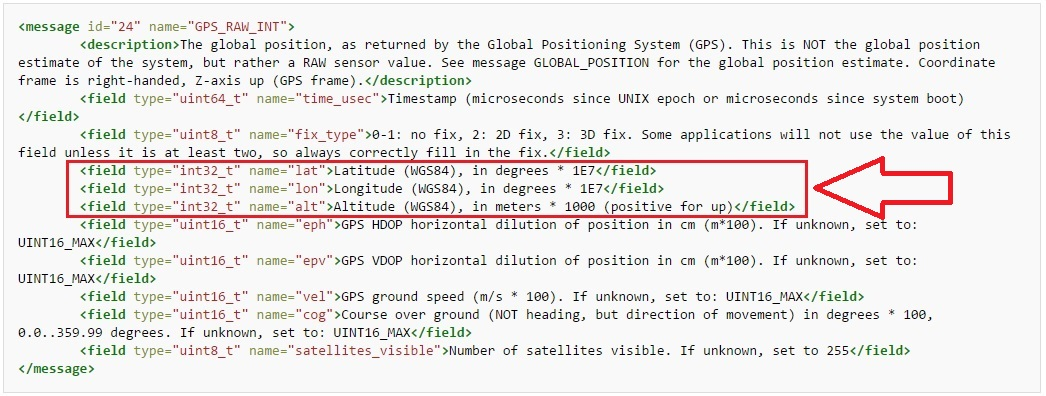
\includegraphics[scale=0.5]{figures/mavlink_msg.jpg}
	\caption{Example of a MAVLink message XML document}
	\label{fig:mav_msg}
\end{figure}

To be noted that the XML document describes the logical ordering of the fields for the protocol, not the actual wire format.

\subsection{Advantages}
To sum up, the MAVLink presents the following advantages:
\begin{itemize}
	\item Small packet size
	\item Message verification
	\item Low bandwidth allocation
	\item Useful at low communication scenario
\end{itemize}

In conclusion, taking the advantages presented above that the MAVLink protocol is a viable option in the case of the UAS at hand.
